% V22 overview, traced to reconstruction_v22/operator.py (current repository snapshot).
% The input JSON is a configuration illustration, not a saved per-point diagnostic.
% Compile: tectonic fig01_pipeline.tex
\documentclass[tikz,border=3mm]{standalone}
\usepackage{fontspec}
\setmainfont{Times New Roman}
\setmonofont{Consolas}
\usepackage{amsmath}
\usetikzlibrary{arrows.meta,calc,positioning}
\definecolor{mainblue}{HTML}{3778A8}
\definecolor{mainorange}{HTML}{CB7736}
\definecolor{ink}{HTML}{25313C}
\definecolor{muted}{HTML}{64717C}
\definecolor{rulegray}{HTML}{BFC6CC}
\definecolor{papergray}{HTML}{F4F5F6}
\begin{document}
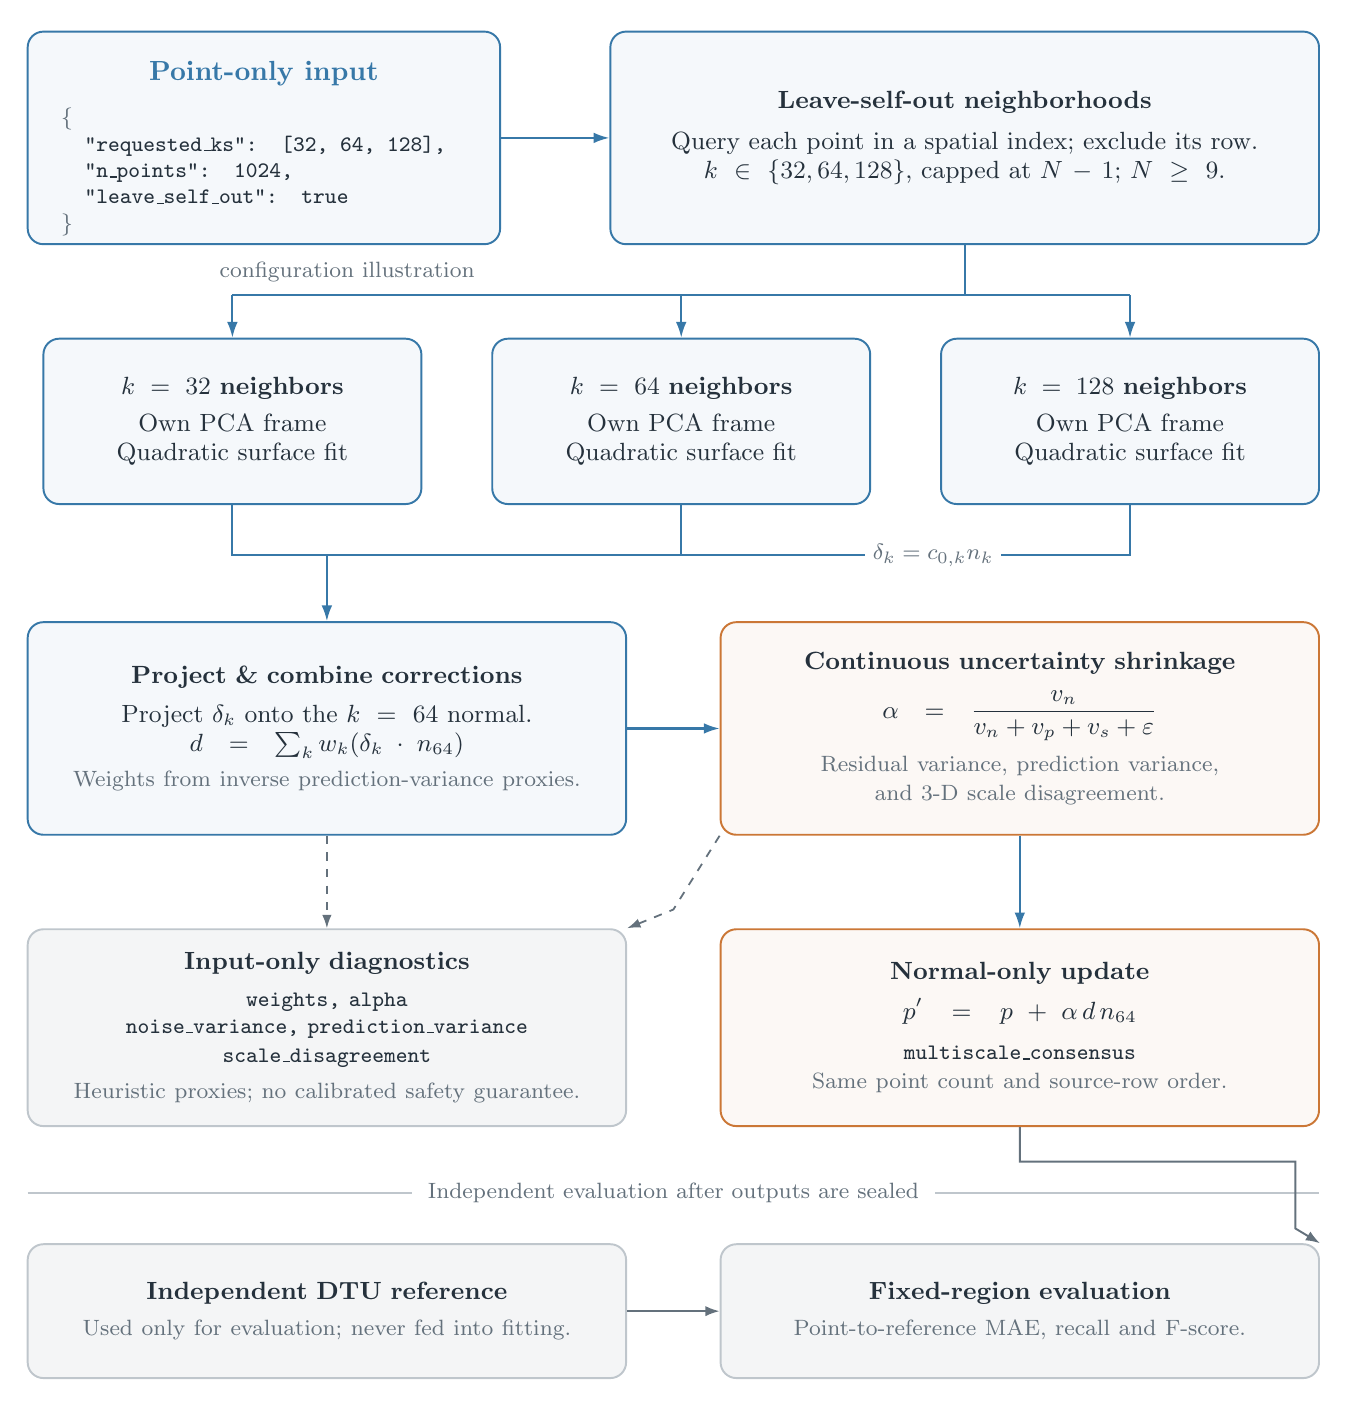
\begin{tikzpicture}[x=1mm,y=1mm,
  font=\fontsize{9}{10.4}\selectfont, text=ink,
  box/.style={draw=mainblue,line width=.7pt,rounded corners=2mm,
              fill=white,align=center,inner sep=2mm},
  bluebox/.style={box,fill=mainblue!5},
  orangebox/.style={box,draw=mainorange,fill=mainorange!5},
  quietbox/.style={box,draw=rulegray,fill=papergray},
  flow/.style={-{Latex[length=2mm,width=1.35mm]},draw=mainblue,line width=.75pt},
  diagnostic/.style={-{Latex[length=1.7mm,width=1.2mm]},draw=muted,line width=.65pt,dashed},
  evalflow/.style={-{Latex[length=1.8mm,width=1.3mm]},draw=muted,line width=.7pt},
  small/.style={font=\fontsize{8}{9.4}\selectfont},
  tinycode/.style={font=\ttfamily\fontsize{7.9}{9.5}\selectfont,align=left}
]
% All visible geometry is within a 164 mm width; 3 mm borders give a 170 mm PDF.
\path[use as bounding box] (0,14) rectangle (164,-158);

\node[bluebox,minimum width=60mm,minimum height=27mm] (input) at (30,0) {};
\node[anchor=north,font=\bfseries\fontsize{10}{11}\selectfont,text=mainblue] at (30,11) {Point-only input};
\node[tinycode,anchor=north west] at (3,5) {\textcolor{muted}{\{}\\
  \quad"requested\_ks": [32, 64, 128],\\
  \quad"n\_points": 1024,\\
  \quad"leave\_self\_out": true\\
  \textcolor{muted}{\}}};
\node[anchor=north east,small,text=muted] at (58,-14.5) {configuration illustration};

\node[bluebox,minimum width=90mm,minimum height=27mm,text width=83mm] (neighbors) at (119,0)
  {\textbf{Leave-self-out neighborhoods}\\[1.5mm]
   Query each point in a spatial index; exclude its row.\\
   $k\in\{32,64,128\}$, capped at $N-1$; $N\geq9$.};
\draw[flow] (input.east) -- (neighbors.west);

\node[bluebox,minimum width=48mm,minimum height=21mm,text width=43mm] (fit32) at (26,-36)
  {\textbf{$k=32$ neighbors}\\[1mm]Own PCA frame\\Quadratic surface fit};
\node[bluebox,minimum width=48mm,minimum height=21mm,text width=43mm] (fit64) at (83,-36)
  {\textbf{$k=64$ neighbors}\\[1mm]Own PCA frame\\Quadratic surface fit};
\node[bluebox,minimum width=48mm,minimum height=21mm,text width=43mm] (fit128) at (140,-36)
  {\textbf{$k=128$ neighbors}\\[1mm]Own PCA frame\\Quadratic surface fit};
\draw[draw=mainblue,line width=.75pt] (neighbors.south) -- (119,-20) -- (26,-20);
\draw[draw=mainblue,line width=.75pt] (119,-20) -- (140,-20);
\foreach \x/\target in {26/fit32,83/fit64,140/fit128}{\draw[flow] (\x,-20) -- (\target.north);}

\draw[draw=mainblue,line width=.75pt] (fit32.south) -- (26,-53) -- (140,-53) -- (fit128.south);
\draw[draw=mainblue,line width=.75pt] (fit64.south) -- (83,-53);
\node[small,fill=white,inner xsep=1mm,inner ysep=.4mm,text=muted] at (115,-53)
  {$\delta_k=c_{0,k}n_k$};

\node[bluebox,minimum width=76mm,minimum height=27mm,text width=69mm] (combine) at (38,-75)
  {\textbf{Project \& combine corrections}\\[1.3mm]
  Project $\delta_k$ onto the $k=64$ normal.\\
  $d=\sum_k w_k(\delta_k\cdot n_{64})$\\[.8mm]
  \textcolor{muted}{\fontsize{8}{9.4}\selectfont Weights from inverse prediction-variance proxies.}};
\draw[flow] (38,-53) -- (combine.north);

\node[orangebox,minimum width=76mm,minimum height=27mm,text width=69mm] (shrink) at (126,-75)
  {\textbf{Continuous uncertainty shrinkage}\\[1.8mm]
  $\displaystyle\alpha=\frac{v_n}{v_n+v_p+v_s+\varepsilon}$\\[1.6mm]
  \textcolor{muted}{\fontsize{8}{9.4}\selectfont Residual variance, prediction variance,\\and 3-D scale disagreement.}};
\draw[flow] (combine.east) -- (shrink.west);

\node[quietbox,minimum width=76mm,minimum height=25mm,text width=69mm] (diag) at (38,-113)
  {\textbf{Input-only diagnostics}\\[1.4mm]
  {\ttfamily\fontsize{8}{9.5}\selectfont weights, alpha\\
  noise\_variance, prediction\_variance\\
  scale\_disagreement}\\[1mm]
  \textcolor{muted}{\fontsize{8}{9.4}\selectfont Heuristic proxies; no calibrated safety guarantee.}};
\node[orangebox,minimum width=76mm,minimum height=25mm,text width=69mm] (output) at (126,-113)
  {\textbf{Normal-only update}\\[1.4mm]
  $\displaystyle p'=p+\alpha\,d\,n_{64}$\\[1.4mm]
  {\ttfamily\fontsize{8}{9.4}\selectfont multiscale\_consensus}\\
  \textcolor{muted}{\fontsize{8}{9.4}\selectfont Same point count and source-row order.}};
\draw[flow] (shrink.south) -- (output.north);
\draw[diagnostic] (combine.south) -- (diag.north);
\draw[diagnostic] (shrink.south west) -- (82,-98) -- (diag.north east);

\draw[rulegray,line width=.5pt] (0,-134) -- (164,-134);
\node[small,fill=white,inner xsep=2mm,text=muted] at (82,-134)
  {Independent evaluation after outputs are sealed};
\node[quietbox,minimum width=76mm,minimum height=17mm,text width=69mm] (reference) at (38,-149)
  {\textbf{Independent DTU reference}\\[1mm]
  \textcolor{muted}{\fontsize{8}{9.4}\selectfont Used only for evaluation; never fed into fitting.}};
\node[quietbox,minimum width=76mm,minimum height=17mm,text width=69mm] (evaluation) at (126,-149)
  {\textbf{Fixed-region evaluation}\\[1mm]
  \textcolor{muted}{\fontsize{8}{9.4}\selectfont Point-to-reference MAE, recall and F-score.}};
\draw[evalflow] (reference.east) -- (evaluation.west);
\draw[evalflow] (output.south) -- (126,-130) -- (161,-130) -- (161,-138.5) -- (evaluation.north east);
\end{tikzpicture}
\end{document}
